

\begin{frame}{$R^0$ -- runnable code}

  \begin{figure}
    \centering
    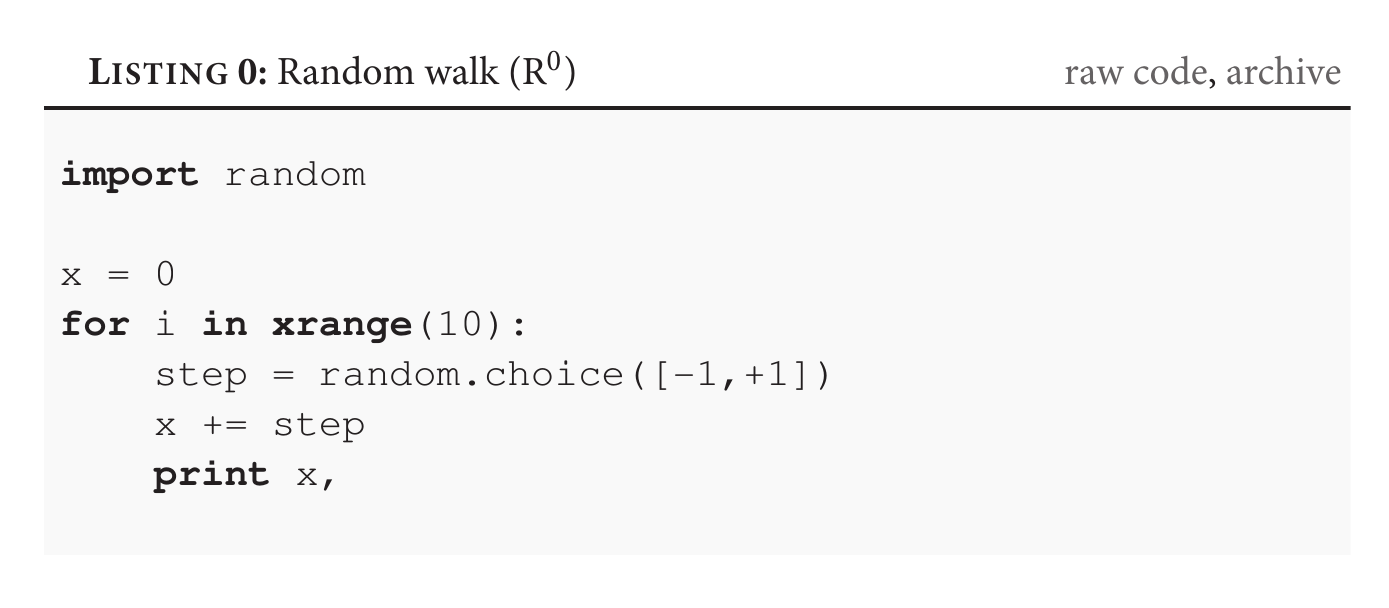
\includegraphics[width=\textwidth]{%
      img/R0_code.png} %
  \end{figure}

  \begin{figure}
    \centering
    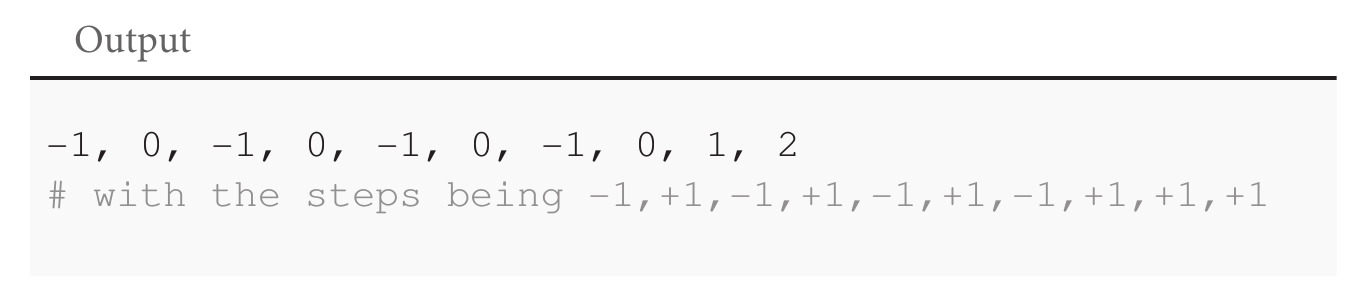
\includegraphics[width=\textwidth]{%
      img/R0_output.png} %
  \end{figure}

  \vspace{1.5cm}  

  \source{\cite{Benureau2018}}
  
  
\end{frame}



\begin{frame}{$R^1$ -- Re-runnable}

  \begin{figure}
    \centering
    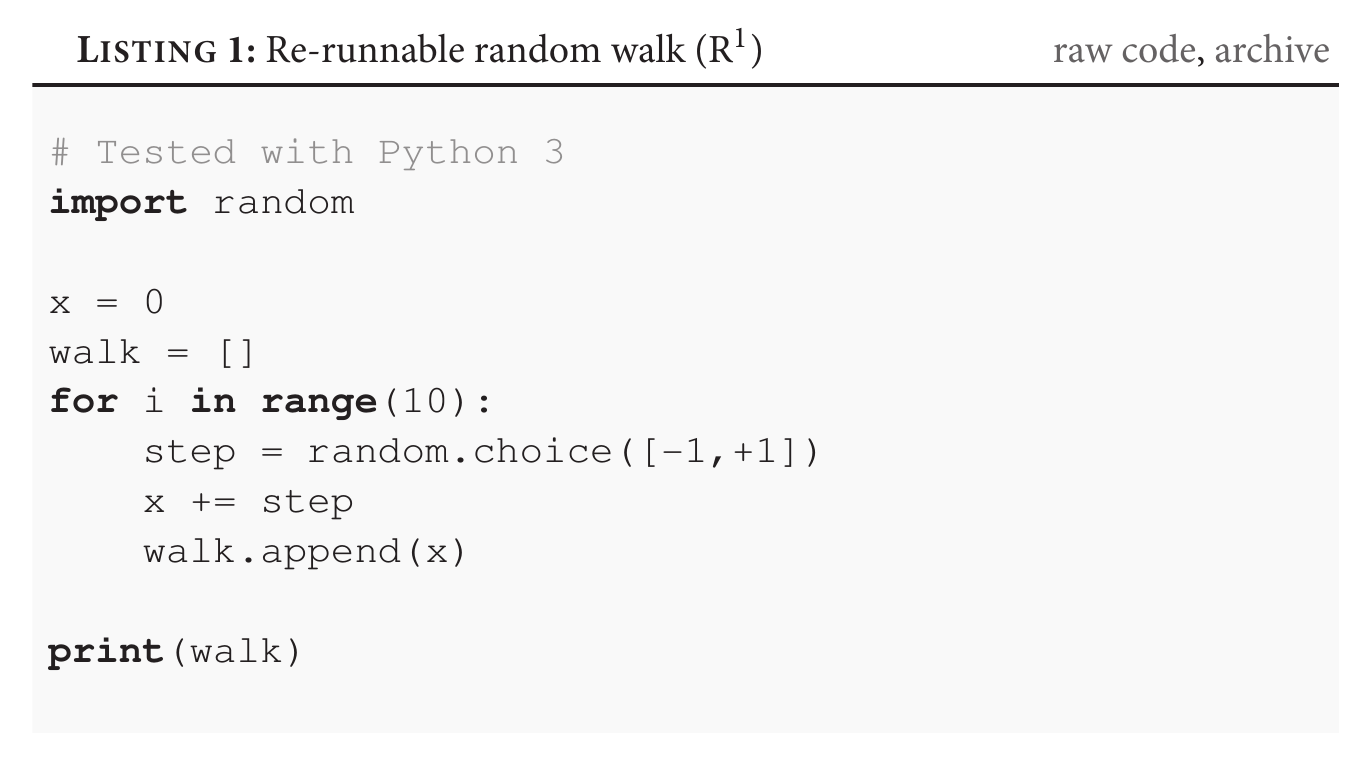
\includegraphics[width=\textwidth]{%
      img/R1_code.png} %
  \end{figure} 
  
  
\end{frame}



\begin{frame}{$R^2$ -- Repeatable}
  
    \begin{figure}
    \centering
    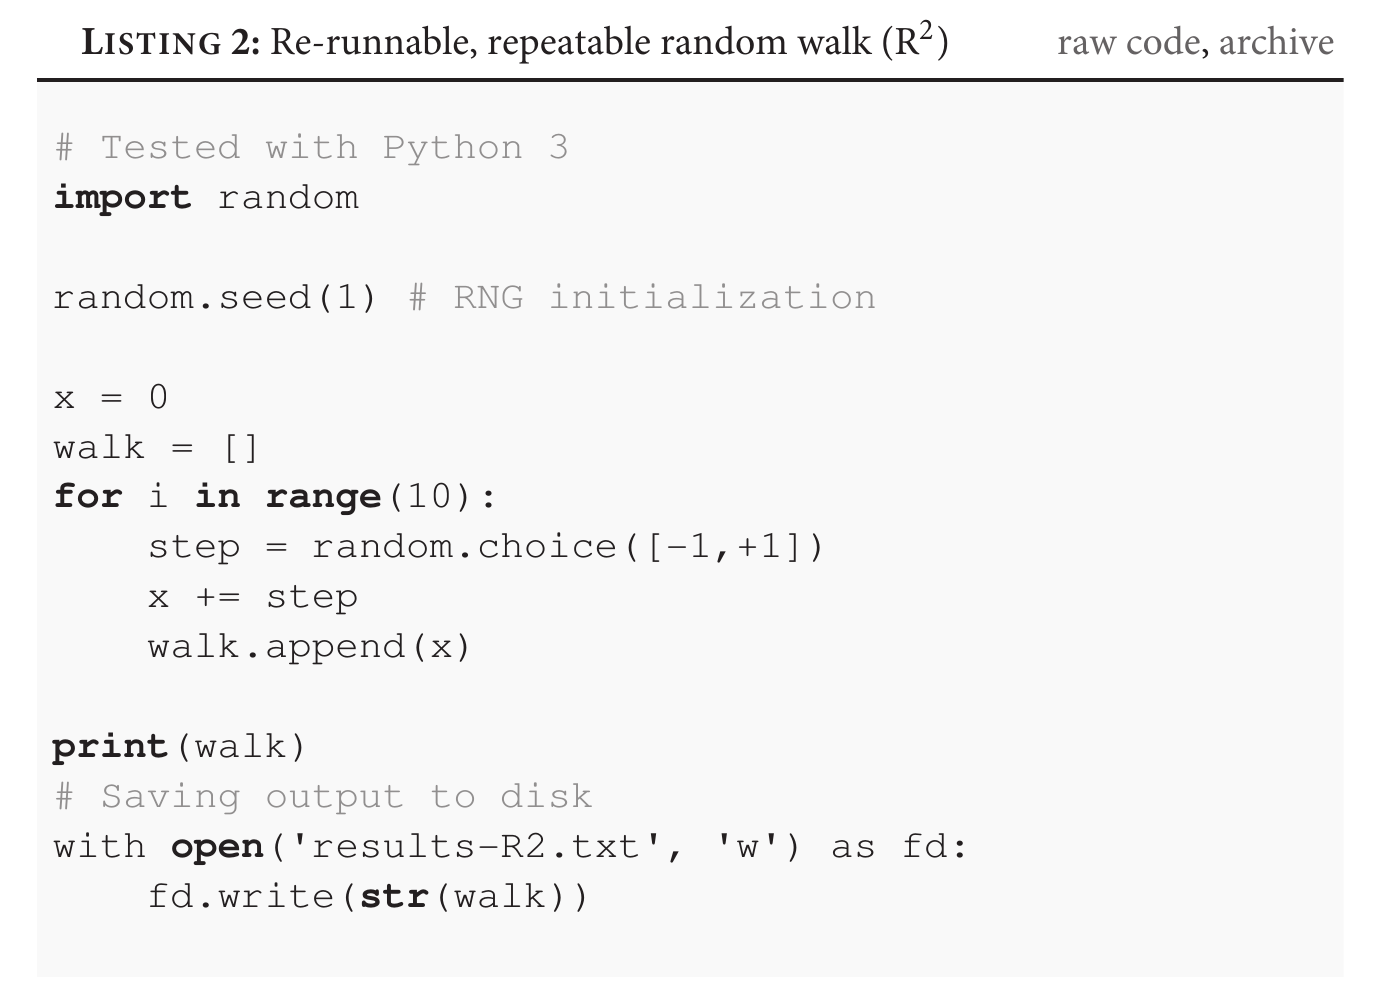
\includegraphics[width=\textwidth]{%
      img/R2_code.png} %
    \end{figure} 
      
\end{frame}



\begin{frame}{$R^3$ -- Reproducible}

  \begin{figure}
    \centering
    \includegraphics<1>[width=.8\textwidth]{%
      img/R3_code01.png} %
    \includegraphics<2>[width=.8\textwidth]{%
      img/R3_code02.png} %   
  \end{figure}

  \source{\only<1>{1}\only<2>{2}/2}
    
\end{frame}


\begin{frame}{$R^4$ -- Reusable}

  \begin{figure}
    \centering
    \includegraphics<1>[width=.8\textwidth]{%
      img/R4_code01.png} %
    \includegraphics<2>[width=.8\textwidth]{%
      img/R4_code02.png} %
    \includegraphics<3>[width=.8\textwidth]{%
      img/R4_code03.png} %   
  \end{figure}

    \source{\only<1>{1}\only<2>{2}\only<3>{3}/3}
    
\end{frame}



\begin{frame}{$R^5$ -- Replicable}

  \begin{figure}
    \centering
    \includegraphics<1>[width=.8\textwidth]{%
      img/R5_code01.png} %
    \includegraphics<2>[width=.8\textwidth]{%
      img/R5_code02.png} %   
  \end{figure}

  \source{\only<1>{1}\only<2>{2}/2}
    
\end{frame}


\begin{frame}{But also...}
  
  \begin{figure}
    \centering
    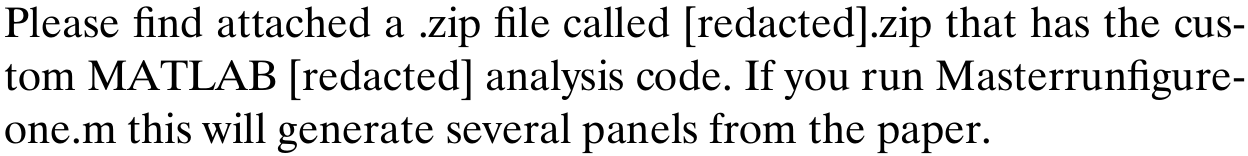
\includegraphics[width=0.95\textwidth]{%
      img/stodden2018_re4.png} %
  \end{figure}

  \begin{figure}
    \centering
    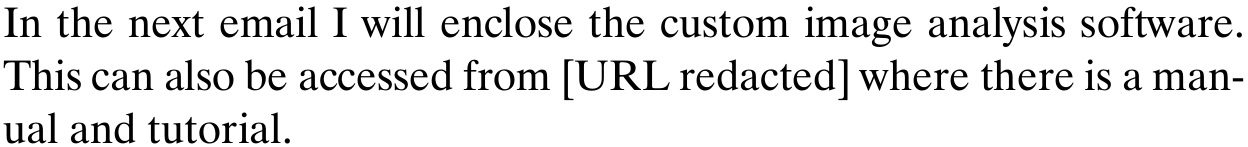
\includegraphics[width=0.95\textwidth]{%
      img/stodden2018_re5.png} %
  \end{figure}

  \begin{figure}
    \centering
    
\includegraphics[width=0.95\textwidth]{%
      img/stodden2018_re6.png} %
  \end{figure}

  \source{\cite{Stodden2018}}
  
\end{frame}



\begin{frame}{Reproducibility when code was available}

  \vspace{0.05cm}
  
  56 out of 91 studies were judged as \textit{potentially reproducible}

  \vspace{0.1cm}

  \only<1-3>{
    \begin{figure}
      \centering
      \includegraphics<1>[width=0.825\textwidth]{%
        img/stodden2018_table4_1-3.png} %
      \includegraphics<2>[width=0.825\textwidth]{%
        img/stodden2018_table4_2-3.png} %
      \includegraphics<3>[width=0.825\textwidth]{%
        img/stodden2018_table4_3-3.png} %
  \end{figure}}

  \only<4>{
    \begin{center}
      \begin{tikzpicture}[every text node part/.style={align=center}]
        \draw (0, 0) node[inner sep=0] {\includegraphics<4>[width=0.825\textwidth]{%
            img/stodden2018_table4_3-3.png}};
        \draw  (0, -2.25) node {Even when code was available, more than half of studies\\ were reproducible only with \textit{\textcolor{red}{significant effort!}}};
      \end{tikzpicture}
  
    \end{center}
  }

  \source{\cite{Stodden2018}}
  
  
  
  
\end{frame}


\begin{frame}{\large Measuring Reproducibility in Computer Systems Research}

  \begin{figure}
    \centering
    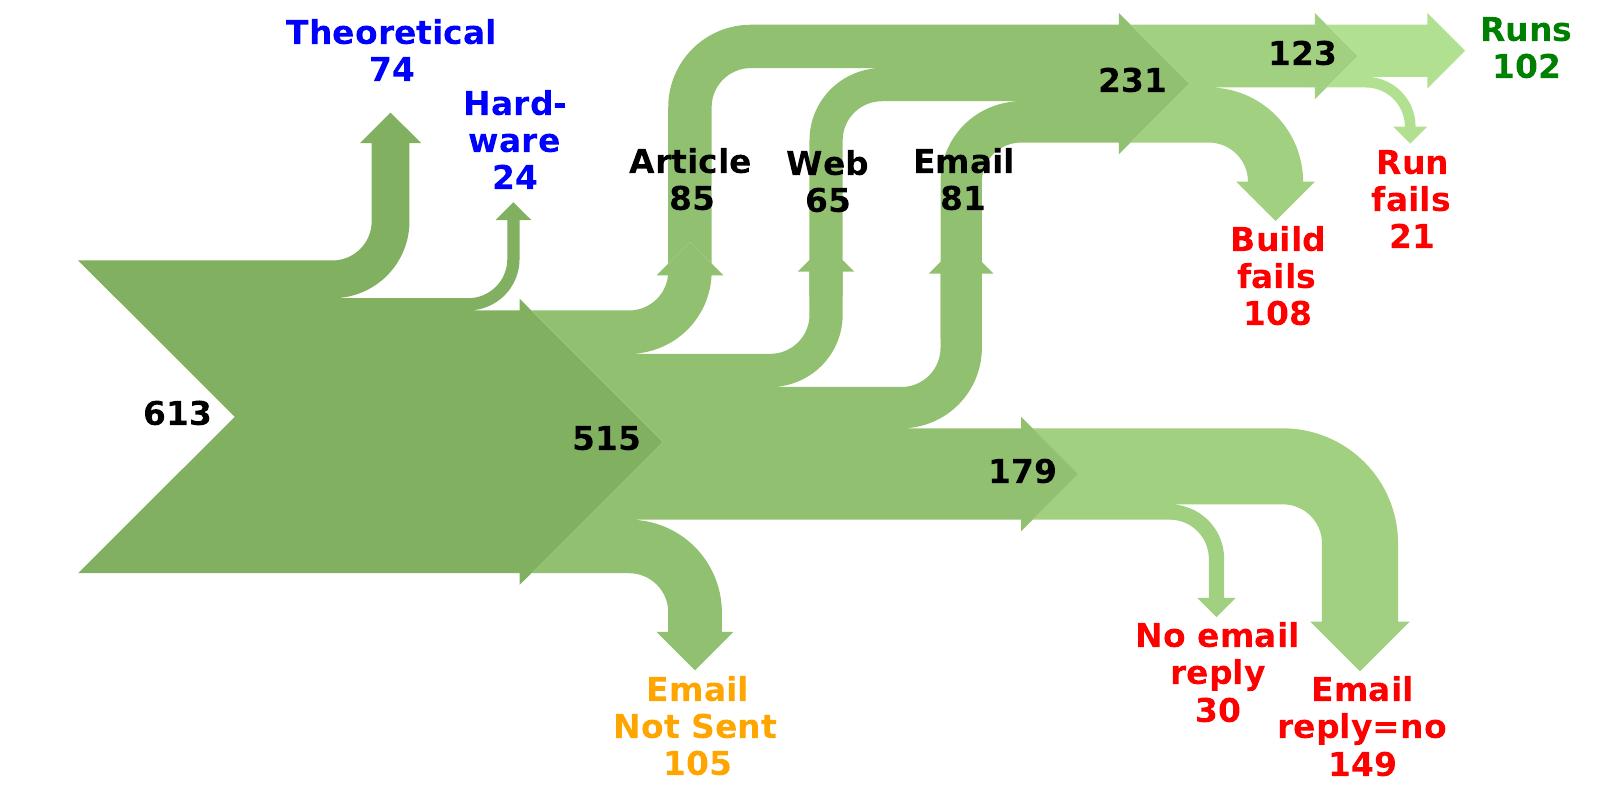
\includegraphics[width=\textwidth]{%
      img/collberg2013_results3.png} %
  \end{figure}
  

  \source{\cite{Collberg2013}}

  \pnote{
    
    613 papers from \\
    - 8 conferences \\
    - 5 journals

    30 minutes of programmer time to try \\
    make build compile/run
    
    Orange: Don't send more than one email to any author \\
    (if author had multiple publications)

    Even if build runs does not even try verify results! \\
    How many more papers will fall off?
    
  }
  
  
\end{frame}
